\documentclass[11pt,a4paper]{article}

% These are extra packages that you might need for writing the equations:
\usepackage{amsmath}
\usepackage{amsfonts}
\usepackage{amssymb}
\usepackage{booktabs}
\usepackage{hyperref}
\usepackage{listings}
\usepackage{xcolor}
\lstset {language=C++,
		 basicstyle=\ttfamily,
         keywordstyle=\color{blue}\ttfamily,
         stringstyle=\color{red}\ttfamily,
         commentstyle=\color{purple}\ttfamily,
         morecomment=[l][\color{magenta}]{\#},
       	 basicstyle=\tiny}

% You need the following package in order to include figures in your report:
\usepackage{graphicx}

% With this package you can set the size of the margins manually:
\usepackage[left=2cm,right=2cm,top=2cm,bottom=2cm]{geometry}


\begin{document}

% Enter the exercise number, your name and date here:
\noindent\parbox{\linewidth}{
 \parbox{.25\linewidth}{ \large ICP, Exercise 06 }\hfill
 \parbox{.5\linewidth}{\begin{center} \large Beat Hubmann \end{center}}\hfill
 \parbox{.2\linewidth}{\begin{flushright} \large Nov 7, 2018 \end{flushright}}
}
\noindent\rule{\linewidth}{2pt}


\section{Introduction}

The single spin flip Metropolis algorithm was implemented as an example Monte Carlo method to simulate
the 2-D Ising model. Energy and Magnetization of the system were measured at different temperatures for two different
system sizes.

\section{Algorithm Description}
The algorithm is implemented as originally published~\cite{metropolis} and as described in the lecture notes~\cite{herrmann}.
Specific to the 2D Ising model, a new configuration is generated by randomly flipping the spin of a lattice element
and then calculating the system's post-change energy.
The dimensionless energy $E$ and magnetization $M$ are calculated as indicated in equations~\ref{eqn:1}~and\ref{eqn:2}, where
$S_i \in \{-1, +1\}$ stands for 'spin down' respectively 'spin up' at site $i$ and $N$~stands for the total number of sites in
the 2D lattice under consideration.
The implemented version of the algorithm allows for 100 system sweeps after each increasing temperature step,
after which every tenth value for $E$ and $M$ is measured during another 100 system sweeps and then averaged to obtain
the respective site values. By doing so, any correlation between measurements should be minimized.

\begin{equation}
	E = -J \cdot \sum_{<i, j>}S_i S_j
\label{eqn:1}
\end{equation}


\begin{equation}
	M = \frac{1}{N}\sum_{i=1}^{N}S_i
\label{eqn:2}
\end{equation}


\section{Results}

The program was implemented as described above and submitted with this report. 
For all experiments, the coupling constant $J$ was fixed to the simplest ferromagnetic value of $J=1.0$. The temperature $T$
was varied in the range from $1$ to $5$ $J/k_B$. No cold starts were used.
The experiment was run twice for 2D Ising lattice side lengths $L \in \{100, 200\}$. The results for dimensionless energy $E$ and magnetization $M$
 for the two lattie sizes are shown in figure~\ref{fig:1}.
The site values between the two different system sizes agree while the larger system shows smoother behaviour as one would expect.
By implementing several of the suggested algorithm options, the run time of the simulation could be kept
in the order of magnitude of minutes.

\begin{figure}[ht]
\begin{center}
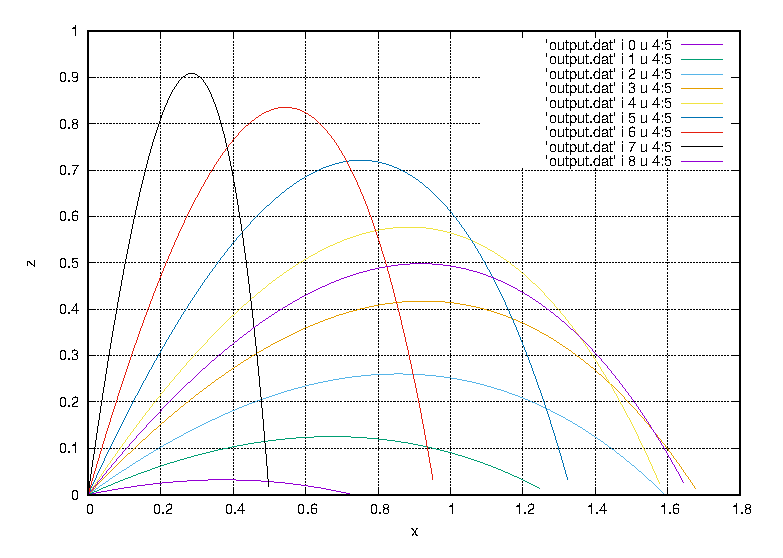
\includegraphics[scale=1.4]{figure1.eps} 
\end{center}
\caption{Value of magnetization $M$ and energy $E$ at different temperatures $T$ according to Metropolis MC with $J=1$ on lattices of side length $L$.}
\label{fig:1}
\end{figure}


\section{Discussion}
As expected, the magnetization $M$ drops off steeply at the critical temperature $T_c = \frac{2}{\log(1+\sqrt{2})} \quad [J/k_B]$.
Also in line width expectations, the energy increases with temperature with the steepest ascent also around $T_c$.





\pagebreak
\begin{thebibliography}{99}


\bibitem{metropolis}
Metropolis, N.,
Rosenbluth, A.W.,
Rosenbluth, M.N.,
Teller, A.H.,
Teller, E.\\
\emph{Equations of State Calculations by Fast Computing Machines},\\
Journal of Chemical Physics. 21 (6): 1087,\\
1953.


\bibitem{herrmann}
	Herrmann, H. J.,
	Singer, H. M.,
	Mueller L.,
	Buchmann, M.-A.,\\
	\emph{Introduction to Computational Physics - Lecture Notes},\\
	ETH Zurich,\\
	2017.


\end{thebibliography}

\end{document}